\documentclass[11pt,a4paper]{article}
\usepackage{epsfig}
\usepackage{amsthm, amssymb}
\usepackage[utf8]{inputenc}
\usepackage{color}
\usepackage[fleqn]{amsmath}
\usepackage{float,tikz}
\usepackage{amssymb, amsfonts, amsthm, booktabs,wasysym}
\usepackage[hidelinks]{hyperref}
\usepackage{verbatim}
\usepackage{tabularx}
\usepackage{graphicx}
\usepackage{longtable}
\usepackage{subcaption}
\usepackage[round]{natbib}


\newcommand{\fnurl}[2]{\footnote{\url{#1} (last accessed: #2)}} %URL als Fussnote
\newcommand{\TODO}[1]{{\color{red}\fbox{#1}}\PackageWarning{TODO}{**** TODO (page \thepage): #1 ****}}

% correct bad hyphenation here
\hyphenation{ana-ly-sis net-work}

%
\begin{document}
\title{
  {\small Bioinformatics II, 2015 \hfill project 3, \today}\\
   Atomic Contact Energies
}

\author{
    Max Emil Sch{\"o}n, Adrian Gei{\ss}ler
}

% make the title area
\maketitle


%\begin{abstract}
%\end{abstract}


\section{Introduction}
Energy functions are used to model protein 3D structures. Aspects that influence
the free energy of proteins are van-der-Waals forces, electrostatics, dipole
interactions, and torsions.
The free desolation energy describes the required energy for the trans-location
of in water solved atoms to the interior of a protein \citep{Zhang1997}, which
therefore is measure for the stability of a structure.
\citet{Zhang1997} described a method to approximate
the desolvation energy based on atom contacts, rather than residue interactions, as proposed by \citet{Miyazawa1996}.

Their approach is to assign one of 18 atom types to each heavy atom. Based on these types, the energetic contribution of each contact pair to the overall energy is derived. A contact pair is defined by \citet{Zhang1997} as two atoms that have a distance below 6\,\AA\ and that are at least ten covalent bonds away from each other. The covalent distance is approximated with respect to connectivity classes without considering bonds in side-chains.

Here, we implement this algorithm and assess its quality on various protein prediction data sets.

\section{Material and Methods}
We implemented the algorithm in the Python language. In addition, we used Biopython's pdb processing functionality \citep{pdb}.

The pairwise contact energies were adopted from \citet{Zhang1997}. We used the
author's cutoff distance of 6\,\AA, because we were able to verify this value
based on the atomic packaging of a large set of non-homologous experimental
protein structures (see \autoref{distance})

The performance of the implemented function was assessed on a subset of the
submissions to the eleventh CASP competition (Critical Assessment of protein
Structure Prediction) \fnurl{http://www.predictioncenter.org/casp11}{\today}.
The datasets in question were T0762, T0769, T0776, T0784. We evaluated each
prediction by superimposing its backbone C$\alpha$ atoms onto the reference and
computing the RMSD values, which we compared to the RMSD numbers listed on the CASP
website~\fnurl{http://www.predictioncenter.org/casp11/local\_acc\_plot.cgi?target=T0762-D1}{\today}.
Afterwards, we investigated correlations between the RMSD and the computed
energies whereby the implementations of
the Pearson and the Spearman correlation coefficients from
the python package SciPy \citep{scipy} were used.

\section{Results}
For every target structure, we visualized the prediction with the lowest RMSD and
the one with the lowest free contact energy in BALLView \citep{ballview}.
Representative visualizations for the datasets T0679 and T0784 are shown in Fig. \ref{fig:visualize}


The relationship between ranked contact energy prediction and the RMSD are shown in Fig. \ref{ranks}.


Pearson's correlation coefficients between the free contact energies and the
RMSD
%AG: NOPE
%calculated by the CASP experiment
ranged from 0.19 to 0.44.
In contrast to these values,
%When comparing our energies to the corresponding ranks from CASP, the
Spearman's rank correlation coefficients were lower, in a range from 0.15 to 0.33 (Table \ref{tbl:comparison}).
A comparison of the $C\alpha$ superimposed RMSD values with the reference values
from
%We also manually compared our RSMD calculations with those from
CASP an high degree of similarity.
%and found that they largely correspond well to one another.

\begin{table}[tbp]
    \caption{\label{tbl:comparison}For the dataset \texttt{T0784} and
        \texttt{T0769}, the tables
        show the computed contact energies and the RMSD counterparts sorted by
        energies (left) and by RMSD (right).}
    \scriptsize
    \centerline{
        \begin{tabular}{|c|c|c|}
            \hline
            \texttt{T0784} & Energy in $\frac{kcal}{mol}$ & RMSD\\
            \hline
            T0784TS156\_1 & $-130.48$ & $1.15$\\
            T0784TS420\_1 & $-127.74$ & $1.17$\\
            T0784TS499\_1 & $-149.46$ & $1.18$\\
            T0784TS237\_1 & $-139.99$ & $1.22$\\
            T0784TS268\_1 & $-160.82$ & $1.28$\\
            \hline
        \end{tabular}
        \begin{tabular}{|c|c|c|}
            \hline
            \texttt{T0784} & Energy in $\frac{kcal}{mol}$ & RMSD\\
            \hline
            T0784TS117\_1 & $-230.12$ & $1.73$\\
            T0784TS008\_1 & $-203.16$ & $1.86$\\
            T0784TS251\_1 & $-193.6 $ & $1.63$\\
            T0784TS038\_1 & $-162.31$ & $1.38$\\
            T0784TS268\_1 & $-160.82$ & $1.28$\\
            \hline
        \end{tabular}
    }

    \vspace{2em}
    \centerline{
        \begin{tabular}{|c|c|c|}
            \hline
            \texttt{T0769} & Energy in $\frac{kcal}{mol}$ & RMSD\\
            \hline
            T0769TS241\_1 & $-59.34$ & $2.67$\\
            T0769TS368\_1 & $-66.75$ & $3.16$\\
            T0769TS258\_1 & $-74.39$ & $4.37$\\
            T0769TS361\_1 & $-79.04$ & $4.41$\\
            T0769TS186\_1 & $-79.97$ & $4.51$\\
            \hline
        \end{tabular}
        \begin{tabular}{|c|c|c|}
            \hline
            \texttt{T0769} & Energy in $\frac{kcal}{mol}$ & RMSD\\
            \hline
            T0769TS442\_1 & $-90.73$ & $16.72$\\
            T0769TS155\_1 & $-90.62$ & $17.12$\\
            T0769TS044\_1 & $-84.32$ & $10.38$\\
            T0769TS169\_1 & $-81.02$ & $10.39$\\
            T0769TS317\_1 & $-80.61$ & $ 6.89$\\
            \hline
        \end{tabular}
    }
\end{table}

%Our results verify the cutoff-distance of 6\,\AA\ chosen by \citet{Zhang1997}, computed from atomic packing densities (Fig. \ref{distance}).
\begin{figure}[tbp]
    \begin{center}
        \begin{subfigure}{.4\textwidth}
            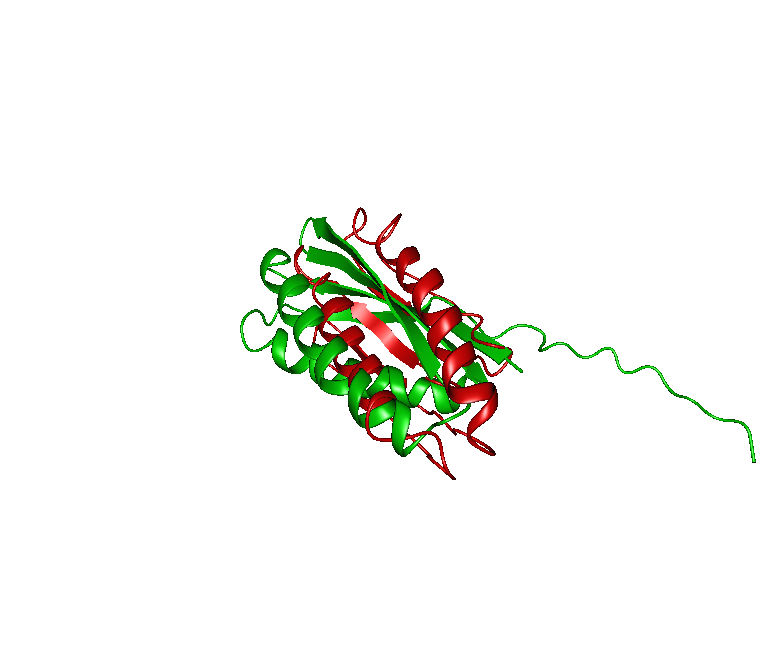
\includegraphics[width=\textwidth]{figures/T0769TS442}
            \subcaption{T0769 442}
        \end{subfigure}
        \begin{subfigure}{.4\textwidth}
            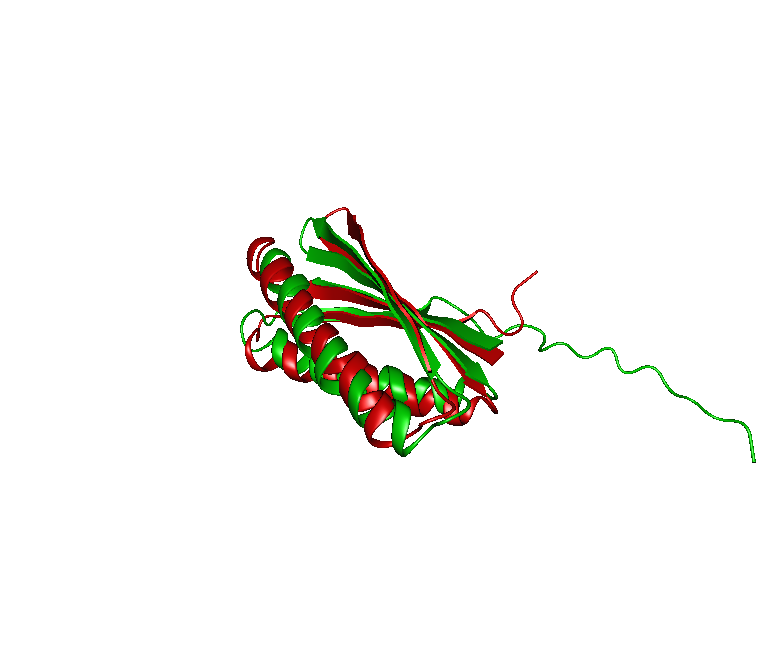
\includegraphics[width=\textwidth]{figures/T0769TS241}
            \subcaption{T0769 241}
        \end{subfigure}

        \begin{subfigure}{.4\textwidth}
            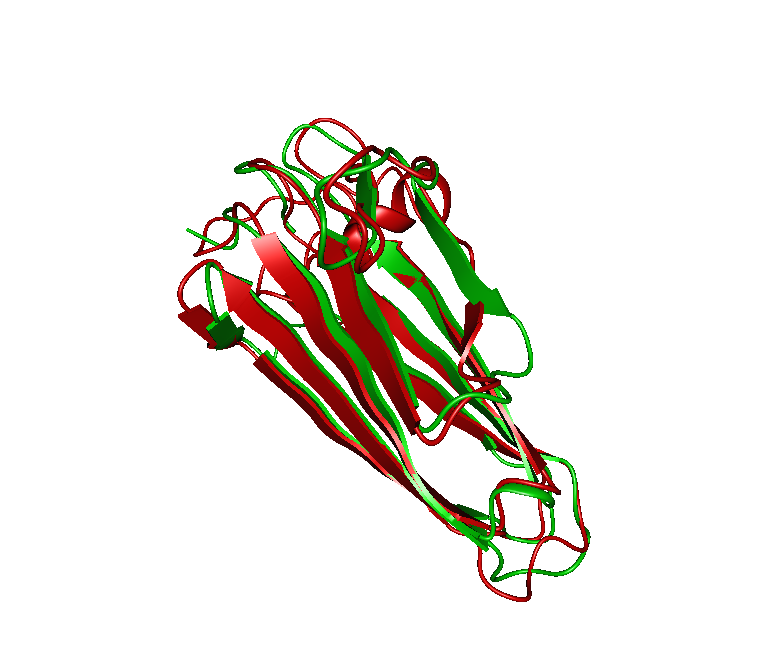
\includegraphics[width=\textwidth]{figures/T0784TS117}
            \subcaption{T0784 117}
        \end{subfigure}
        \begin{subfigure}{.4\textwidth}
            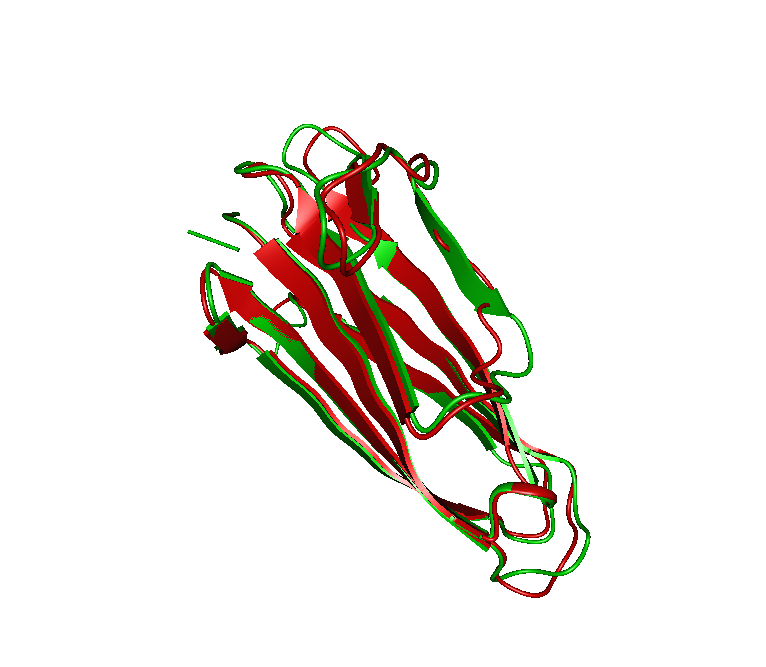
\includegraphics[width=\textwidth]{figures/T0784TS156}
            \subcaption{T0784 156}
        \end{subfigure}
    \end{center}
    \caption{Best scoring predictions of T0769 and T0784 evaluated using (a,c) atomic contact energies and (b,d) the RMSD between prediction and experimental structure. green: target experimental stucture. red: predicted structure.}
    \label{fig:visualize}
\end{figure}
\begin{figure}[tbp]%[!h]
    \centering
    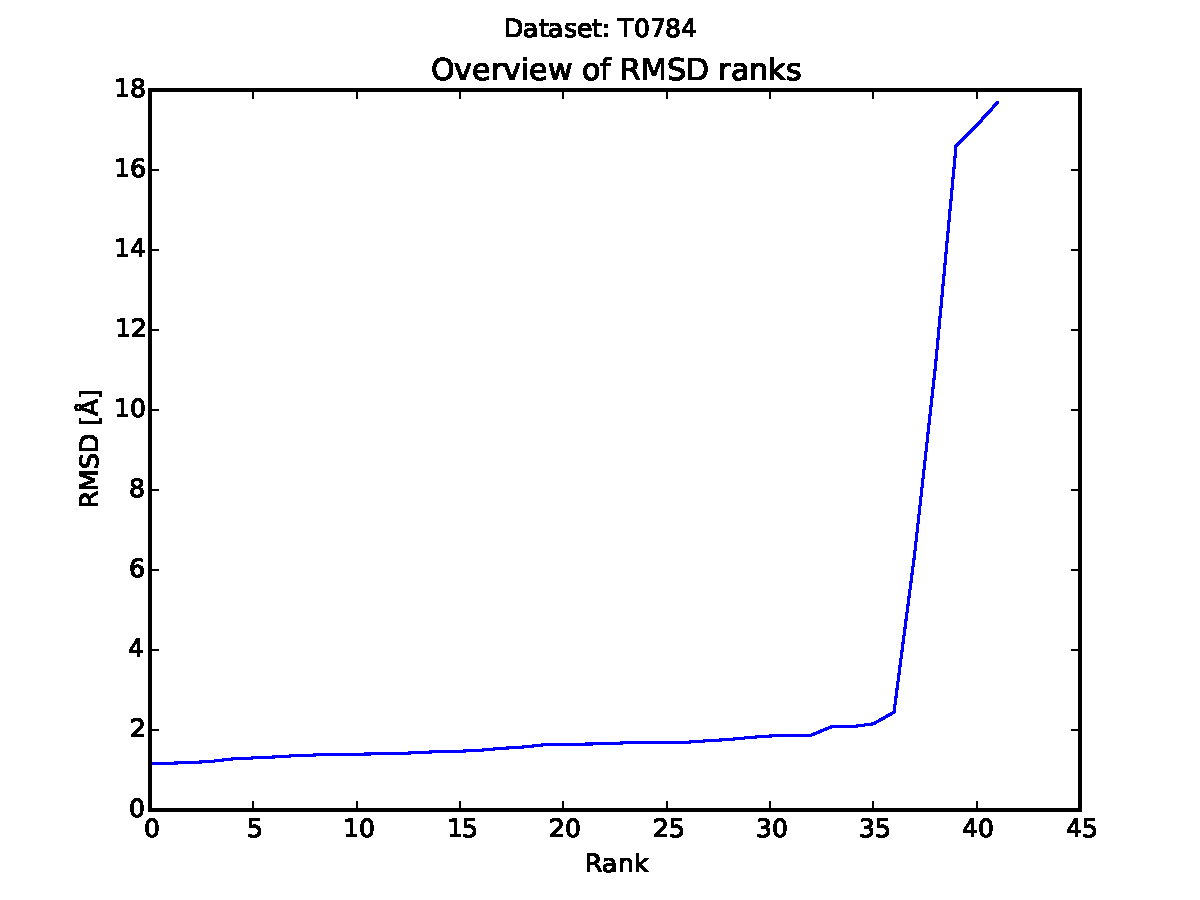
\includegraphics[width=.7\textwidth]{../results/rank_T0784}
    \caption{Calculated RMSD values are plotted against the rank of the
        corresponding prediction
        %in the original CASP11 experiment
        for the target set
        \texttt{T0784}.}
    \label{ranks}
\end{figure}
\begin{figure}[tbp]%[!h]
    \centering
    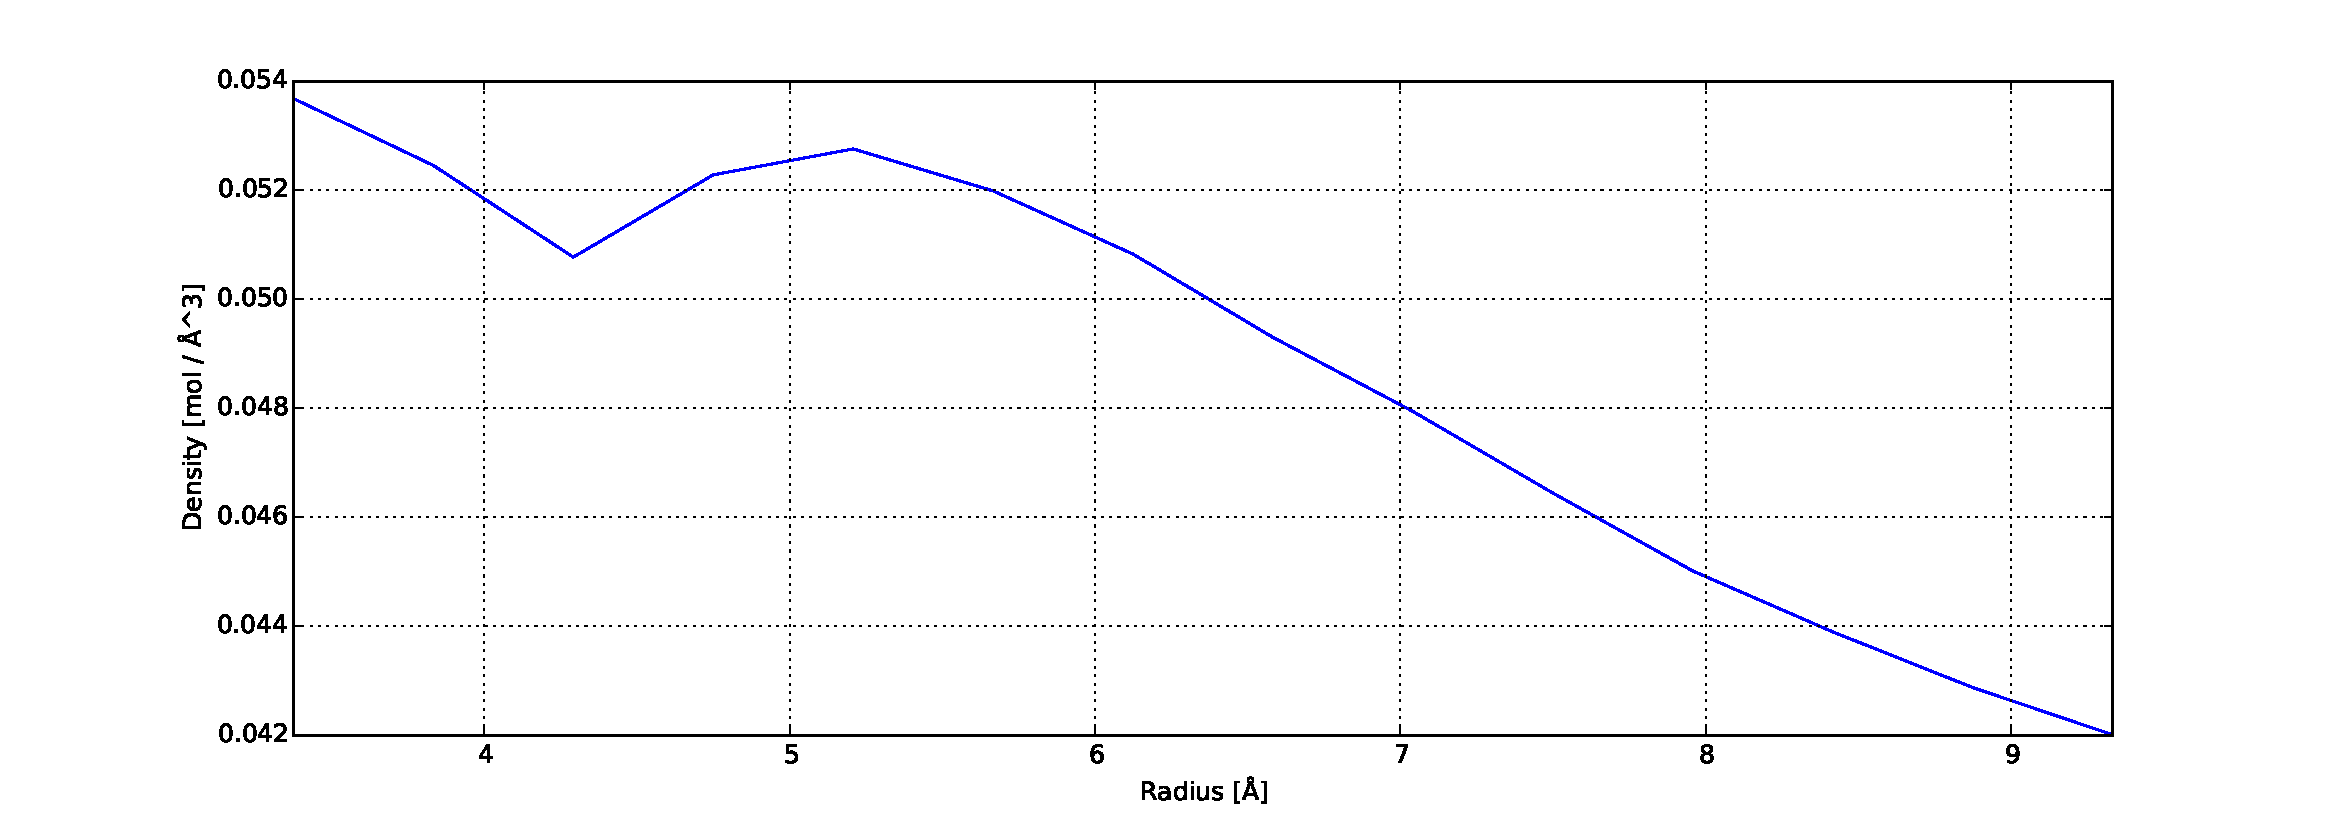
\includegraphics[width=1\textwidth]{figures/better.pdf}
    \caption{Shown is the atomic packaging estimated by the number density
    according to a radius around an interior atom. An atom is considered to be
    buried if the accessible surface area (SAS) is zero.}
    \label{distance}
\end{figure}



\section{Discussion}

% - Threshold
After implementing the algorithm of \citet{Zhang1997}, we were able to reproduce
the threshold value of $6$\,\AA\ on a non-homologous structure set.
%This value is in so far justified, since it considers the
A relative increase of density
for radii around this value
%around this radius range
was observable (see \autoref{distance}) which could be
due to the relevance for atomic contacts.
% - RMSD different
The correlation metrics Pearson and Spearman did not indicate a linear
correlation between RMSD and the computed energies.
However, visual inspections 
of the RMSD distribution suggest that these metrics are bound to fail, because
significant changes were only observed for the lower ranking third of the
predicted structures.
% - suitability of correlation
The original CASP11 evaluations take this property of RMSD into account, as they utilize a multitude of other quality measures.
% - Trends

Although the correlation coefficients are low, plots of the superimposed
structures show trends of consensus with the reference structures.
% - Idea 18 years old
% - not random, but not good

Since the overall energy is derived from the sum of contact energies,
the implemented algorithm just took a few minutes on the whole dataset.
Therefore, we suggest that the energy function of \citet{Zhang1997} is suitable
to quickly assess the quality of folds, even though the resulting values will not
be able to compete with more current free desolation energy functions.

%As shown by Fig. \ref{ranks}, RMSD values change little for the predictions
%which scored highest in the original CASP11 experiment. Together with the fact
%that the prediction with lowest energy in no case possesed the lowest RMSD as
%well, this suggests that the RMSD measure is a rather poor assessment for
%prediction quality on its own. Further it seems that the best scoring
%predictions are not far away from each other in most cases.\\

%\begin{table}
\caption{results for predictions on T0762. Best energy and rmsd are marked in bold.}
\begin{tabular}{lll}
PDB & RMSD & Energy in kcal/mol\\\hline
T0762TS008\_1.pdb & 2.3423191305 & \textbf{-262.8469047619}\\
T0762TS011\_1.pdb & 2.7698841026 & -168.9030476191\\
T0762TS022\_1.pdb & 2.5058039439 & -162.9670952381\\
T0762TS038\_1.pdb & 2.5708829119 & -191.4314285714\\
T0762TS041\_1.pdb & 2.4066233264 & -247.9363333333\\
T0762TS050\_1.pdb & 2.9965283038 & -179.2812380952\\
T0762TS073\_1.pdb & 2.5517540142 & -180.0836666667\\
T0762TS117\_1.pdb & 2.7479596589 & -152.076952381\\
T0762TS133\_1.pdb & 2.4481363601 & -175.1629047619\\
T0762TS145\_1.pdb & 2.6966658285 & -126.8349047619\\
T0762TS156\_1.pdb & 2.3042503171 & -190.0696666667\\
T0762TS160\_1.pdb & 3.263572163 & -152.7326190476\\
T0762TS171\_1.pdb & 3.4890752584 & -138.0823809524\\
T0762TS184\_1.pdb & 2.2928815484 & -188.3076666667\\
T0762TS193\_1.pdb & 2.4744865096 & -174.6419047619\\
T0762TS206\_1.pdb & 3.134063264 & -144.5034285714\\
T0762TS210\_1.pdb & 2.5129260903 & -142.9043809524\\
T0762TS212\_1.pdb & 2.1513475418 & -166.0571904762\\
T0762TS216\_1.pdb & 2.4099770382 & -154.2829047619\\
T0762TS228\_1.pdb & 9.385668499 & -142.7432380952\\
T0762TS237\_1.pdb & 2.9223547684 & -169.5801428572\\
T0762TS251\_1.pdb & \textbf{2.0353168441} & -198.3766666667\\
T0762TS263\_1.pdb & 2.6020588681 & -168.0090476191\\
T0762TS268\_1.pdb & 2.8247720358 & -180.3427142857\\
T0762TS277\_1.pdb & 2.0999864471 & -160.3694285714\\
T0762TS279\_1.pdb & 2.8014960162 & -157.4457619048\\
T0762TS300\_1.pdb & 2.6303333034 & -186.3836190476\\
T0762TS335\_1.pdb & 4.4916672191 & -188.3896190476\\
T0762TS345\_1.pdb & 8.1449379541 & -187.4612380952\\
T0762TS346\_1.pdb & 2.8014960162 & -157.4457619048\\
T0762TS349\_1.pdb & 2.5729844986 & -176.5188095238\\
T0762TS381\_1.pdb & 4.0131846845 & -142.8844285714\\
T0762TS410\_1.pdb & 2.2182007065 & -162.9987142857\\
T0762TS414\_1.pdb & 4.2846602592 & -181.4261428572\\
T0762TS420\_1.pdb & 2.7646056492 & -171.873952381\\
T0762TS436\_1.pdb & 2.9020538844 & -165.2876190476\\
T0762TS448\_1.pdb & 2.8999667601 & -162.2623809524\\
T0762TS452\_1.pdb & 4.8824693376 & -187.9945714286\\
T0762TS454\_1.pdb & 7.8411398975 & -137.1416190476\\
T0762TS479\_1.pdb & 2.7188284869 & -159.5322857143\\
T0762TS492\_1.pdb & 2.8928415675 & -170.923\\
T0762TS499\_1.pdb & 2.2102185447 & -143.9080476191
\end{tabular}
\end{table}


\begin{longtable}{lll}
\caption{results on T079, best energy and rmsd are labeled in bold}
\endfirsthead PDB & RMSD & Energy in kcal/mol\\\hline
\endhead PDB & RMSD & Energy in kcal/mol\\\hline
T0769TS006\_1.pdb & 20.1730457219 & 9.9426666667\\
T0769TS008\_1.pdb & 7.656606437 & -47.6180952381\\
T0769TS011\_1.pdb & 7.90669551 & -53.1626666667\\
T0769TS014\_1.pdb & 7.2800902969 & -78.608047619\\
T0769TS022\_1.pdb & 6.2814170073 & -41.037047619\\
T0769TS024\_1.pdb & 8.1636320221 & -26.2007142857\\
T0769TS026\_1.pdb & 11.5847410454 & -11.5636190476\\
T0769TS032\_1.pdb & 11.0449515749 & -59.215047619\\
T0769TS034\_1.pdb & 12.4326106396 & -39.230047619\\
T0769TS038\_1.pdb & 11.4938620902 & -71.6676190476\\
T0769TS040\_1.pdb & 4.5479075741 & -75.5332857143\\
T0769TS041\_1.pdb & 7.1711046291 & -65.6891904762\\
T0769TS042\_1.pdb & 10.7702826637 & -76.5509047619\\
T0769TS044\_1.pdb & 10.379460472 & -84.324952381\\
T0769TS049\_1.pdb & 6.2149362872 & -46.1097619048\\
T0769TS050\_1.pdb & 8.9607134116 & -65.8122857143\\
T0769TS054\_1.pdb & 7.5130952377 & -67.1312380952\\
T0769TS056\_1.pdb & 10.0754920578 & -65.0741428571\\
T0769TS063\_1.pdb & 16.1141743491 & -67.052047619\\
T0769TS064\_1.pdb & 4.6211297931 & -66.2501904762\\
T0769TS065\_1.pdb & 9.4828543553 & -54.6042380952\\
T0769TS067\_1.pdb & 9.8518281632 & -11.4737619048\\
T0769TS073\_1.pdb & 10.7955344714 & -63.272\\
T0769TS080\_1.pdb & 9.6458158366 & -67.0588571429\\
T0769TS110\_1.pdb & 23.7304577067 & -16.3631904762\\
T0769TS111\_1.pdb & 9.7456809802 & -52.6412380952\\
T0769TS117\_1.pdb & 8.0170568464 & -59.8334761905\\
T0769TS118\_1.pdb & 5.8724940559 & -73.6708095238\\
T0769TS120\_1.pdb & 4.8855322705 & -69.8123333333\\
T0769TS132\_1.pdb & 12.7361139511 & -71.6454761905\\
T0769TS133\_1.pdb & 8.2845850564 & -63.7264761905\\
T0769TS144\_1.pdb & 8.6599310797 & -59.6228095238\\
T0769TS145\_1.pdb & 15.7795153686 & -9.5483333333\\
T0769TS155\_1.pdb & 17.1179459224 & -90.6197619048\\
T0769TS156\_1.pdb & 9.921559656 & -77.6414761905\\
T0769TS157\_1.pdb & 8.7380329701 & -60.2150952381\\
T0769TS160\_1.pdb & 9.1739726894 & -50.0969047619\\
T0769TS162\_1.pdb & 11.4072506411 & -69.2266666667\\
T0769TS169\_1.pdb & 10.388204067 & -81.0181904762\\
T0769TS171\_1.pdb & 9.7614822619 & -50.252047619\\
T0769TS173\_1.pdb & 16.0507642325 & -51.4058095238\\
T0769TS184\_1.pdb & 4.6211297931 & -66.2501904762\\
T0769TS186\_1.pdb & 4.5056666703 & -79.9672380952\\
T0769TS193\_1.pdb & 7.4138503031 & -34.809047619\\
T0769TS197\_1.pdb & 6.5098909593 & -75.0500952381\\
T0769TS203\_1.pdb & 6.1777008534 & -79.8995714286\\
T0769TS204\_1.pdb & 11.4452488091 & -57.5974761905\\
T0769TS210\_1.pdb & 9.3218468239 & -55.165\\
T0769TS212\_1.pdb & 10.6563858985 & -52.5722380952\\
T0769TS216\_1.pdb & 6.7414717331 & -72.8697142857\\
T0769TS228\_1.pdb & 10.7489144331 & -61.8762380952\\
T0769TS230\_1.pdb & 11.7064917635 & -71.1991904762\\
T0769TS235\_1.pdb & 10.3741848392 & -63.1856666667\\
T0769TS237\_1.pdb & 19.7873241656 & -25.9186190476\\
T0769TS241\_1.pdb & \textbf{2.6748016595} & -59.343047619\\
T0769TS251\_1.pdb & 11.4793688956 & -72.1082380952\\
T0769TS258\_1.pdb & 4.3658125828 & -74.3942380952\\
T0769TS260\_1.pdb & 7.5478941478 & -63.680952381\\
T0769TS263\_1.pdb & 6.3583017914 & -60.6837619048\\
T0769TS268\_1.pdb & 12.5206470774 & -59.0740952381\\
T0769TS276\_1.pdb & 9.2283590943 & -48.8672380952\\
T0769TS277\_1.pdb & 8.6187720319 & -66.4583809524\\
T0769TS279\_1.pdb & 7.9277072215 & -69.9848095238\\
T0769TS282\_1.pdb & 4.6205525448 & -65.9706666667\\
T0769TS290\_1.pdb & 8.6787419682 & -79.7527142857\\
T0769TS296\_1.pdb & 5.6087466103 & -58.6694285714\\
T0769TS300\_1.pdb & 10.8891677857 & -55.8492380952\\
T0769TS301\_1.pdb & 8.6187720319 & -66.4583809524\\
T0769TS310\_1.pdb & 6.7827244945 & -69.0379047619\\
T0769TS317\_1.pdb & 6.8894944503 & -80.6148095238\\
T0769TS322\_1.pdb & 6.1114435755 & -51.8862857143\\
T0769TS326\_1.pdb & 8.9346872229 & -66.206047619\\
T0769TS328\_1.pdb & 7.2269895599 & -68.7308095238\\
T0769TS333\_1.pdb & 5.9682157126 & -60.9969047619\\
T0769TS335\_1.pdb & 10.8604551953 & -64.507047619\\
T0769TS336\_1.pdb & 4.8855322705 & -69.8123333333\\
T0769TS338\_1.pdb & 13.758906479 & -69.6464285714\\
T0769TS342\_1.pdb & 6.1261436042 & -73.287047619\\
T0769TS345\_1.pdb & 9.1735222065 & -65.4832380952\\
T0769TS346\_1.pdb & 12.9339727638 & -34.0533333333\\
T0769TS347\_1.pdb & 8.7465818149 & -77.1880952381\\
T0769TS349\_1.pdb & 5.4210657112 & -55.3339047619\\
T0769TS357\_1.pdb & 12.9475028359 & -42.653\\
T0769TS358\_1.pdb & 13.7379987801 & -79.7847619048\\
T0769TS361\_1.pdb & 4.4147342409 & -79.04\\
T0769TS362\_1.pdb & 4.6812316055 & -64.3309047619\\
T0769TS364\_1.pdb & 10.0510151598 & -66.3444285714\\
T0769TS368\_1.pdb & 3.1590900898 & -66.7455238095\\
T0769TS381\_1.pdb & 10.9574952212 & -52.961047619\\
T0769TS386\_1.pdb & 21.4333289559 & -25.2683333333\\
T0769TS391\_1.pdb & 11.7579485804 & -44.0409047619\\
T0769TS403\_1.pdb & 6.2984516357 & -71.4070952381\\
T0769TS410\_1.pdb & 11.3970114047 & -49.1604285714\\
T0769TS414\_1.pdb & 11.0135831182 & -56.553952381\\
T0769TS417\_1.pdb & 10.148918345 & -40.8924285714\\
T0769TS420\_1.pdb & 8.8262360334 & -52.8872857143\\
T0769TS425\_1.pdb & 7.4797328656 & -58.3386666667\\
T0769TS428\_1.pdb & 5.0235525248 & -60.3364285714\\
T0769TS433\_1.pdb & 6.5335668605 & -76.7075714286\\
T0769TS434\_1.pdb & 8.0186462074 & -47.955047619\\
T0769TS436\_1.pdb & 5.4276048278 & -62.4596666667\\
T0769TS437\_1.pdb & 18.0746184973 & -31.9063809524\\
T0769TS438\_1.pdb & 10.1679787487 & -55.886047619\\
T0769TS439\_1.pdb & 7.7351910912 & -72.6902857143\\
T0769TS442\_1.pdb & 16.7228006464 & \textbf{-90.7309047619}\\
T0769TS445\_1.pdb & 6.5098909593 & -75.0500952381\\
T0769TS448\_1.pdb & 10.6652748317 & -65.3305238095\\
T0769TS452\_1.pdb & 10.8839209839 & -52.0201428571\\
T0769TS454\_1.pdb & 8.2663766022 & -36.2377619048\\
T0769TS457\_1.pdb & 6.817524943 & -70.8647619048\\
T0769TS465\_1.pdb & 8.5608396165 & -59.7923333333\\
T0769TS466\_1.pdb & 13.7327026472 & -31.1620952381\\
T0769TS476\_1.pdb & 6.1261436042 & -73.287047619\\
T0769TS479\_1.pdb & 11.6131435105 & -77.7516190476\\
T0769TS482\_1.pdb & 10.0754920578 & -65.0741428571\\
T0769TS483\_1.pdb & 11.7064917635 & -71.1991904762\\
T0769TS492\_1.pdb & 5.4000275617 & -66.2724285714\\
\end{longtable}

%bibliography
\bibliographystyle{abbrvnat}
% argument is your BibTeX string definitions and bibliography database(s)
\bibliography{ref}

\end{document}
